\section{Arduino}

O Arduino Uno e o Arduino Mega são responsáveis pela leitura do registro de ponto. Os dois são interligados por meio das portas seriais. O Arduino Uno é ligado diretamente ao sensor RFID e recebe os bytes informando o valor da tag sempre que uma leitura é realizada. Em seguida, ele transfere esses dados para o Arduino Mega, que envia uma requisição POST ao servidor web, solicitando que o registro de ponto seja criado. De acordo com a resposta do servidor (que pode ser um código HTTP 201 no caso de sucesso, ou 400 para falha), um LED é ligado na protoboard (verde para sucesso ou vermelho para falha). Assim, ao passar cartão, o estudante tem uma resposta visual praticamente imediata. 

Na figura ~\ref{arduino_esquema} é possível notar a simplicidade do projeto: ele conta com apenas alguns pequenos componentes e é bastante flexível. 

\begin{figure}[H]
	\centering
	\caption{Esquema de ligação dos componentes eletrônicos.}
	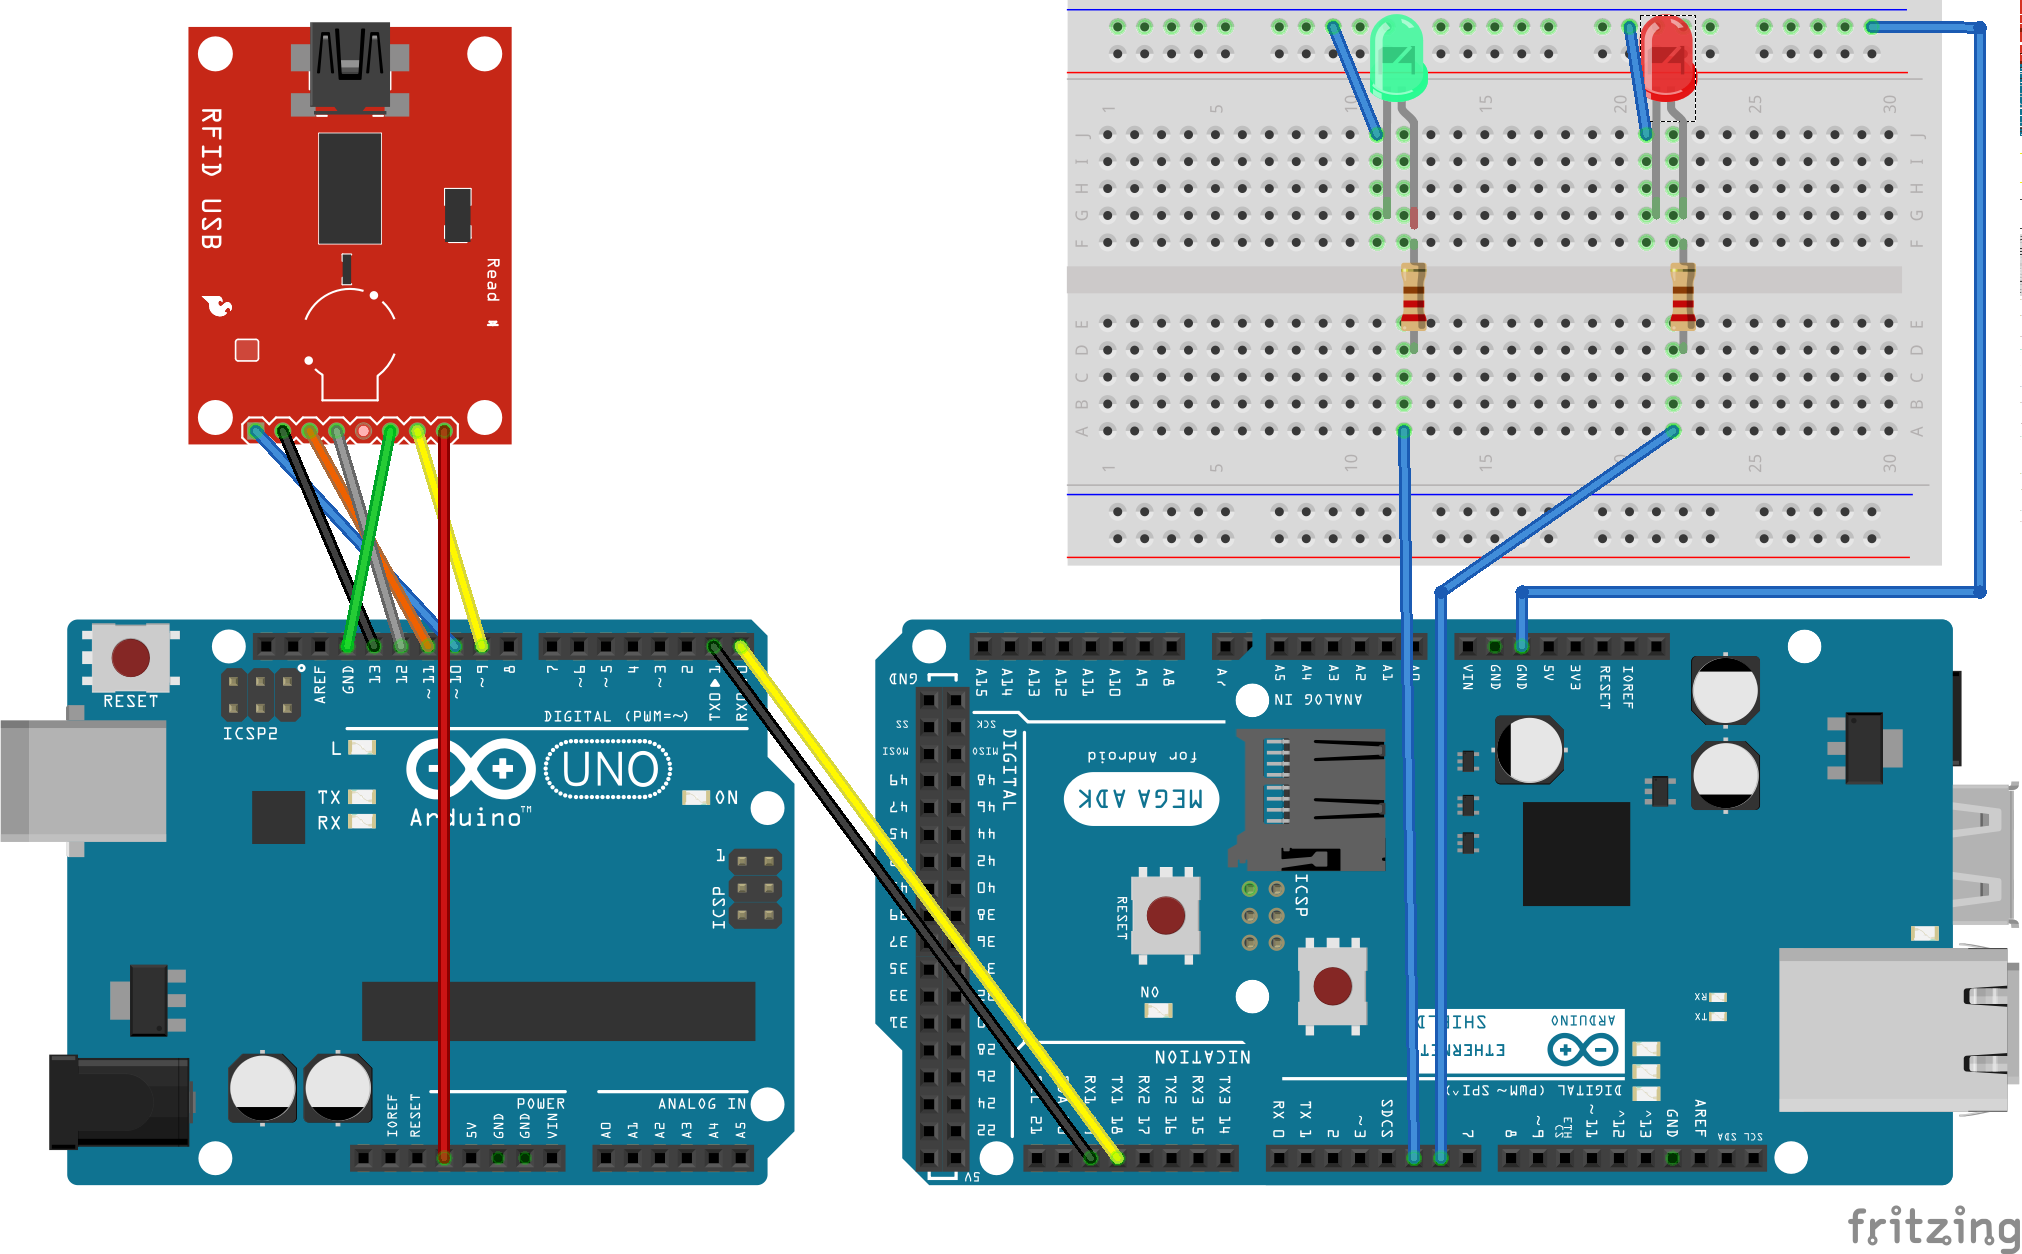
\includegraphics[scale=0.8]{imagens/arduino_esquema.png}
	\label{arduino_esquema}
\end{figure}